
In spite of the high level of agreement observed between theory
calculations and ATLAS top measurements, the top normalization is
constrained using a top-rich control region (CR). The cross section
measurements in
ATLAS,~\cite{bib:ttbar_cross_section,bib:Wt_cross_section}, require
the selected jets to be central ($|\eta|<2.5$), whereas in the VBF
analysis, due to the signal topology, the $\eta$ requirement is looser,
$|\eta|<4.5$. Dedicated top measurements have yet to probe this region
to test existing theoretical models, motivating the use of a
data-driven top estimate. Because the kinematic
shapes are similar for \ttbar~and ST, these processes share a common
normalization. All of the selection cuts applied in the SR are also
applied in the top CR, with the exception of the BJV. Instead of
requiring zero $b$-tags, exactly one $b$-tag is required, enriching
this region with top background while while minimizing contamination from
sources without heavy flavor quarks in the final state. The top CR is
subdivided into BDT bins, and the top
normalization is computed separately in each bin. This approach is
used because the BDT spans a large and relatively unknown region of
phase space, and there is no \textit{a priori} reason to assume that the
normalization is constant across the BDT spectrum. 

The normalization factor (NF) in each BDT bin is the ratio of the number of
top events in the CR in data to number of top events
predicted by MC, expressed as

\begin{equation}
\label{chap:analysis:equation:top_nf}
\tau_i = \frac{N_{data,i}^{CR} - N_{non-top,MC,i}^{CR}}{N_{top,MC,i}^{CR}}
\end{equation}

\noindent where the index $i$ represents the $i^{\textrm{th}}$ BDT bin. The top estimate in the SR is obtained by scaling the MC
prediction by the NF from the CR

\begin{equation}
\begin{aligned}
\label{chap:analysis:equation:top_est}
N_{top,i}^{SR,est} = \tau_i N_{top,MC,i}^{SR}
& = \frac{N_{top,MC,i}^{SR}}{N_{top,MC,i}^{CR}}(N_{data,i}^{CR} -
N_{non-top,MC,i}^{CR}) \\
& \equiv \alpha_i (N_{data,i}^{CR} - N_{non-top,MC,i}^{CR})
\end{aligned}
\end{equation}

\noindent The extrapolation factor $\alpha$ is derived from
MC. The top systematics are obtained by computing the variation in
this quantity. The statistical uncertainty on the top NF is
approximately $\sqrt{N_{data}^{CR}}/N_{top,MC}^{CR}$ which is just
$1/\sqrt{N_{data}^{CR}}$ for a sufficiently pure top CR. More data
events in the CR corresponds to a lower statistical uncertainty on the
top NF. Motivated by this, the top CR is merged for the two flavor
channels \eemm and \emme. Also, because the BDT kinematically rejects
top well, the two high BDT bins are depleted of this process in
the $b$ tag region. To improve the statistical precision, these two
bins are merged in the top CR and a common NF is applied to the two
high BDT SR bins. The event yields and the corresponding top NF are
shown at each cut stage in the top CR in
Table~\ref{chap:analysis:tab:top_cr_cutflow}. Distributions of the BDT
inputs in the top CR without any cut on BDT score are shown in
Figures~\ref{chap:analysis:fig:bdt_inputs_topcr_df}
and~\ref{chap:analysis:fig:bdt_inputs_topcr_sf}. The error bars shown
are MC statistical uncertainties only. These plots illustrate
that \POWHEG+\PYTHIA models \ttbar~remarkably well in this phase space
region. There is a hint of mis-modeling in the \dphill distribution at
low values in both \emme and \eemm channels. This feature is covered
by the uncertainties on the top background. 

\begin{table}
\begin{center}
\renewcommand{\arraystretch}{1.2}
\resizebox{0.8\textwidth}{!}{
\begin{tabular}{ l | c | c | c | c | c }
\hline
         & \ttbar & ST & non-top & data & top NF  \\ \hline
        \Njet$\geq{2}$ & $64944$ & $3571$ & $9895$ & $80986$ & {\color{blue}$1.04 \pm 0.004$} \\
        \Nbjet$=1$ & $21952$ & $1865$ & $2586$ & $27791$ & {\color{blue}$1.06 \pm 0.007$} \\
        CJV & $16455$ & $1521$ & $1912$ & $21071$ & {\color{blue}$1.07 \pm 0.008$} \\
        OLV & $3284 \pm 7$ & $305 \pm 2$ & $344 \pm 10$ & $4183$ & {\color{blue}$1.07 \pm 0.02$} \\
        $Z\rightarrow{\tau \tau}$ veto & $2387 \pm 6$ & $217 \pm 1$ & $184 \pm 7$ & $2964$ & {\color{blue}$1.07 \pm 0.02$} \\
        \textbf{BDT bin 0} & $2305 \pm 6$ & $204 \pm 1.259$ & $169 \pm 7$ & $2807$ & {\color{blue}$1.05 \pm 0.02$} \\
        \textbf{BDT bin 1} & $71.9 \pm 1.0$ & $10.4 \pm 0.4$ & $13.1 \pm 1.1$ & $143$ & {\color{blue}$1.58 \pm 0.15$} \\
        \textbf{BDT bins 2+3} & $10.1 \pm 0.4$ & $2.1 \pm 0.2$ &
        $2.4 \pm 0.4$ & $14$ & {\color{blue}$0.95 \pm 0.31$} \\
        \hline
\end{tabular}
}
\caption[Cutflow in top CR.]{\ttbar, ST, non-top background, and data
        event counts in the top control region. Yields are shown at
        each cutflow stage}
\label{chap:analysis:tab:top_cr_cutflow}
\end{center}
\end{table}

\begin{figure}[h]
  \centering
   \includegraphics[width=0.4\textwidth]{fig/analysis/top_cr_validation/emme_CutTopControl_2jetinclZttVeto_DPhill_mh125_lin.eps}
   \includegraphics[width=0.4\textwidth]{fig/analysis/top_cr_validation/emme_CutTopControl_2jetinclZttVeto_Mll_mh125_lin.eps}
   \includegraphics[width=0.4\textwidth]{fig/analysis/top_cr_validation/emme_CutTopControl_2jetinclZttVeto_DYjj_mh125_lin.eps}
   \includegraphics[width=0.4\textwidth]{fig/analysis/top_cr_validation/emme_CutTopControl_2jetinclZttVeto_Mjj_mh125_lin.eps}
   \includegraphics[width=0.4\textwidth]{fig/analysis/top_cr_validation/emme_CutTopControl_2jetinclZttVeto_Pttot_tr_mh125_lin.eps}
   \includegraphics[width=0.4\textwidth]{fig/analysis/top_cr_validation/emme_CutTopControl_2jetinclZttVeto_MT_tr_mh125_lin.eps}
   \includegraphics[width=0.4\textwidth]{fig/analysis/top_cr_validation/emme_CutTopControl_2jetinclZttVeto_SumOFMvaMLepxJety_mh125_lin.eps}
   \includegraphics[width=0.4\textwidth]{fig/analysis/top_cr_validation/emme_CutTopControl_2jetinclZttVeto_contOLV_mh125_lin.eps}
  % \includegraphics[width=0.32\textwidth]{fig/analysis/top_cr_validation/emme_CutTopControl_2jetinclZttVeto_BDT_8var_mh125_lin.eps}
   \caption{Distributions
   of \dphill, \mll, \dyjj, \mjj, \pTtot, \mT, \SumMlj, and \lepEtaCent
   in the \emme top CR after the $Z\rightarrow{\tau\tau}$ veto.}
  \label{chap:analysis:fig:bdt_inputs_topcr_df}
\end{figure}

\begin{figure}[h]
  \centering
  \includegraphics[width=0.4\textwidth]{fig/analysis/top_cr_validation/eemm_CutTopControl_2jetinclZttVeto_DPhill_mh125_lin.eps}
   \includegraphics[width=0.4\textwidth]{fig/analysis/top_cr_validation/eemm_CutTopControl_2jetinclZttVeto_Mll_mh125_lin.eps}
   \includegraphics[width=0.4\textwidth]{fig/analysis/top_cr_validation/eemm_CutTopControl_2jetinclZttVeto_DYjj_mh125_lin.eps}
   \includegraphics[width=0.4\textwidth]{fig/analysis/top_cr_validation/eemm_CutTopControl_2jetinclZttVeto_Mjj_mh125_lin.eps}
   \includegraphics[width=0.4\textwidth]{fig/analysis/top_cr_validation/eemm_CutTopControl_2jetinclZttVeto_Pttot_tr_mh125_lin.eps}
   \includegraphics[width=0.4\textwidth]{fig/analysis/top_cr_validation/eemm_CutTopControl_2jetinclZttVeto_MT_tr_mh125_lin.eps}
   \includegraphics[width=0.4\textwidth]{fig/analysis/top_cr_validation/eemm_CutTopControl_2jetinclZttVeto_SumOFMvaMLepxJety_mh125_lin.eps}
   \includegraphics[width=0.4\textwidth]{fig/analysis/top_cr_validation/eemm_CutTopControl_2jetinclZttVeto_contOLV_mh125_lin.eps}
   %\includegraphics[width=0.48\textwidth]{fig/analysis/top_cr_validation/eemm_CutTopControl_2jetinclZttVeto_BDT_8var_mh125_lin.eps}
   \caption{Distributions
   of \dphill, \mll, \dyjj, \mjj, \pTtot, \mT, \SumMlj, and \lepEtaCent
   in the \eemm top CR after the $Z\rightarrow{\tau\tau}$ veto.}
  \label{chap:analysis:fig:bdt_inputs_topcr_sf}
\end{figure}

As mentioned above, since the extrapolation factor $\alpha
= \frac{N_{top,MC}^{SR}}{N_{top,MC}^{CR}}$ is determined by MC, the
theoretical systematics on the top background are evaluated by
measuring the variation of this ratio. The uncertainties are binned in
BDT score, accounting for the fact the extrapolation is done
separately in each BDT bin. Four sources of uncertainty
are considered: the parton shower (PS) model, PDF, the QCD scale, and
the matrix element model. For the PS modeling uncertainty, the default
sample with \PYTHIA showering is compared to the same hard scatter
generator but with \HERWIG showering at reconstruction
level. The differences in the BDT spectrum is $<5\%$ in the low BDT
bin and less than the statistical uncertainties in the high BDT
bins. For the uncertainty from the choice of PDF, the \ctten error sets
are used and the uncertainty is \textapprox 1\% across the BDT
spectrum. Uncertainties are of the same order if they are derived by
instead comparing \ctten and \nnpdf. 

The remaining two sources of uncertainty are evaluated at truth
level with the true momentum 4-vectors of the final state particles
after showering and hadronization, but before interacting with the
detector. Truth level quantities are defined to best reflect the
corresponding observable, and are then used as BDT inputs, defining a
``truth-level BDT''. Truth jets are built using the anti-$k_t$
algorithm on truth hadrons instead of topo-clusters, with the same
$p_T$ and \eta~cuts used in the selection of reconstruction level jets. Track \etmiss is
defined using truth tracks from charged, interacting particles that
fall within the tracking volume, $|\eta|<2.47$, where the track selection
efficiency is modeled by a logistic turn-on in track $p_T$. Tracks
that fall within a \dR~of 0.4 of a selected jet are excluded, because
these jets are included in the calculation of \etmiss. Finally,
$b$-tagging is captured by weighting events according to the
probability that the event has zero $b$-tags or one $b$-tag. This
probability can be expressed in terms of the tagging efficiencies

\begin{eqnarray}
        w_{0} &=\; p(0\; \textrm{tag})\; =& \prod_{i} 1
        - \epsilon_{i}(p_T,\eta,fl)  \\
        w_{1} &=\; p(1\; \textrm{tag})\;
        =& \sum_{i} \epsilon_{i}(p_T,\eta,fl) \cdot \prod_{i \neq j}
        (1 - \epsilon_{j}(p_T,\eta,fl)),
\label{chap:analysis:eq:btag_formula}
\end{eqnarray}

\noindent where the $\epsilon_i$ are the tagging efficiencies for the
$i^{\textrm{th}}$ jet. These truth level definitions are validated
against the corresponding reconstruction level quantities, implying
that using the variation induced in the truth BDT is well-motivated for
the extraction of uncertainties. 

The QCD scale uncertainty was evaluated by independently varying the factorization
($\mu_F$) and renormalization ($\mu_R$) scales up and down by a factor
of two in a \ttbar~sample generated with \MCATNLO and showered
with \HERWIG. The largest deviation from the nominal $\alpha$ value is
taken as the uncertainty. This uncertainty ranges from 0\% in the
lowest BDT bin to 5\% in the highest. However, in every bin, the
uncertainty is statistically compatible with zero due to insufficient
MC statistics. 

The largest theoretical uncertainty on top is the matrix element
modeling uncertainty. The difference in the predicted $\alpha$ value
is computed for three generators: \MCATNLO, \POWHEG, and \ALPGEN. The
same PS program, \HERWIG, is used in each case. The largest difference,
observed between \MCATNLO and \ALPGEN, is assigned as the
uncertainty. Figure~\ref{chap:analysis:fig:alpha_ratio} displays the
ratio $\alpha_{\MCATNLO}/\alpha_{\ALPGEN}$ binned in BDT. The deviation
of this ratio from unity is taken as the uncertainty-- 10\%, 12\%, and
21\%, respectively. 

Q: do I want to discuss \MCATNLO as an outlier?

\begin{figure}[h]
  \centering
  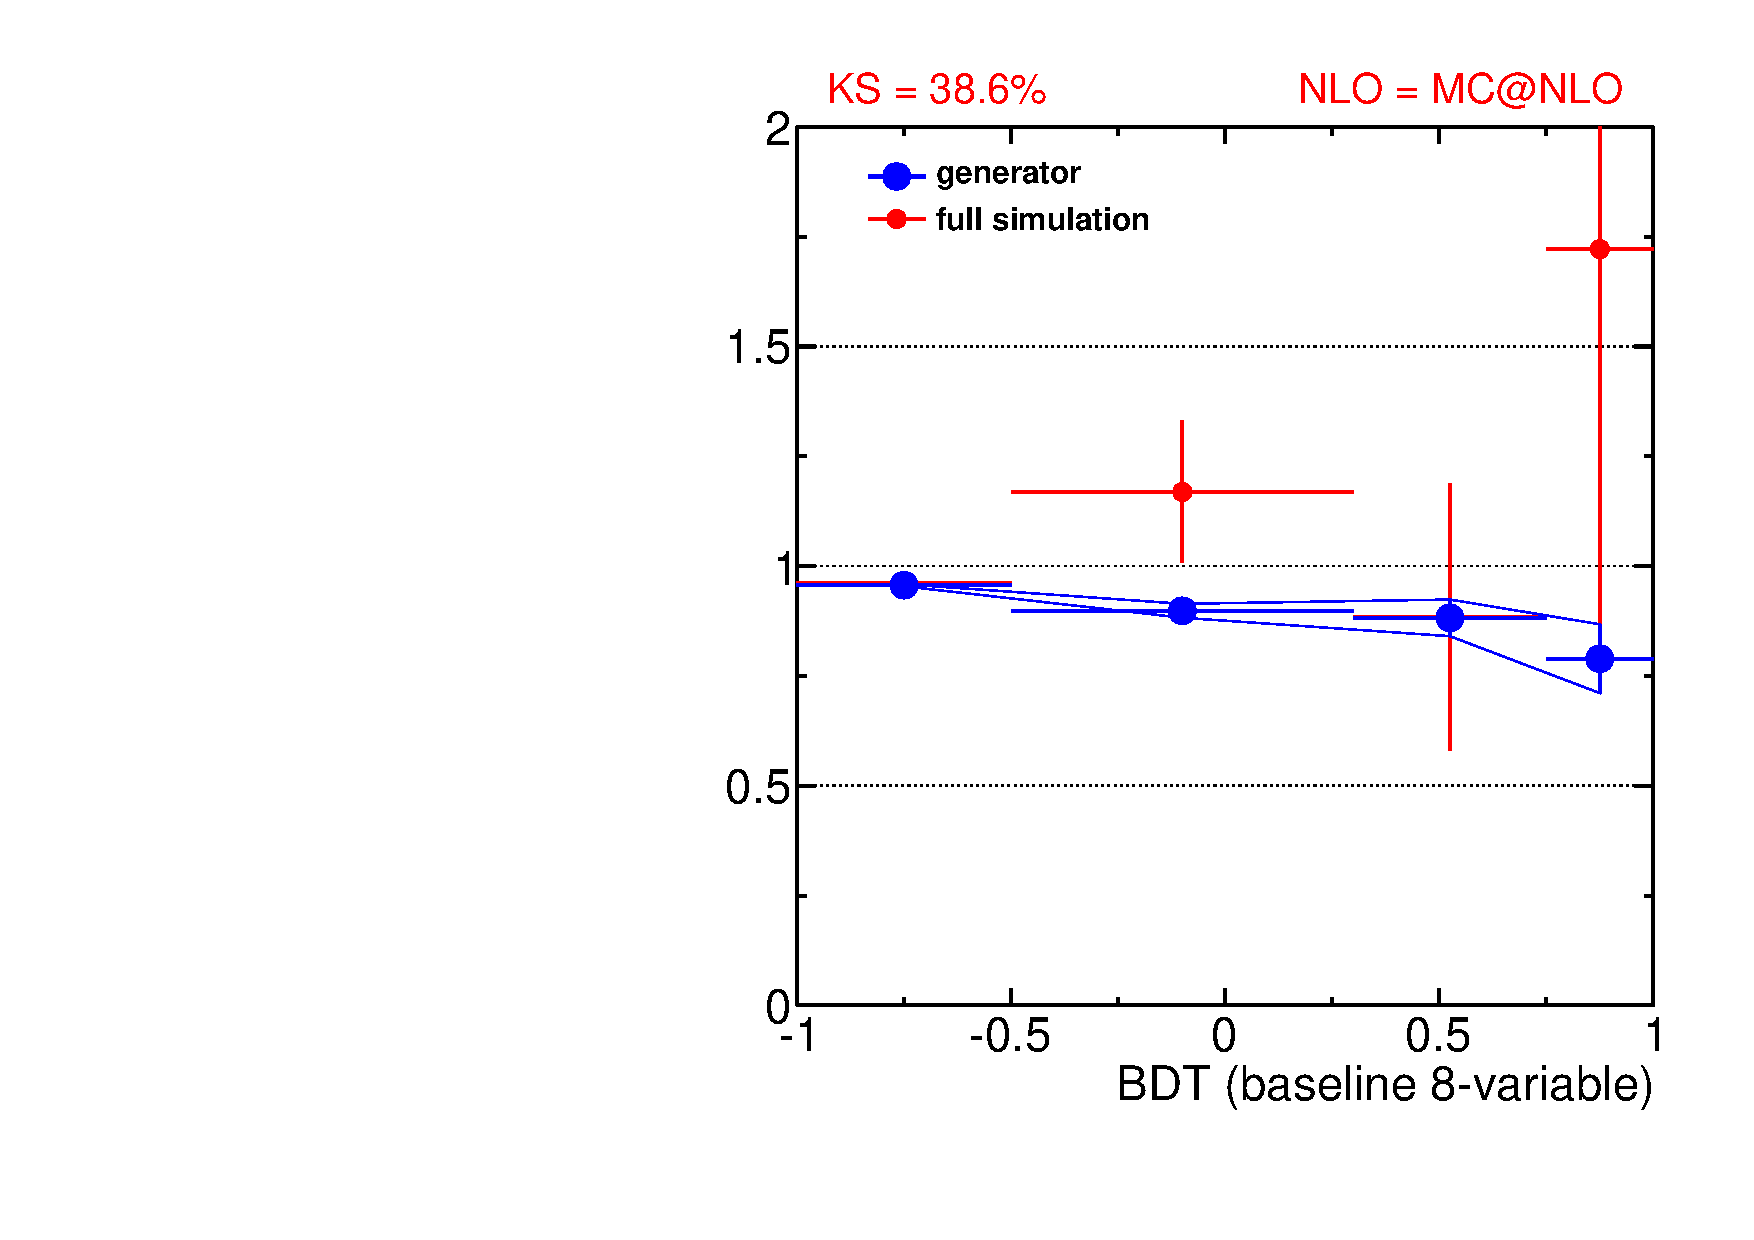
\includegraphics[width=0.6\textwidth]{fig/analysis/ttbar_sys_cjv_mcatnlo03.pdf}
   \caption{Ratio of $\alpha$ predicted by \ALPGEN to that predicted
  by \MCATNLO. Truth level is shown in blue and reconstruction level
  with large statistical uncertainties is shown in red. Difference
  from unity is taken as an uncertainty.}
  \label{chap:analysis:fig:alpha_ratio}
\end{figure}


%\begin{table}
%\begin{center}
%\begin{tabular}{ | l | c | c | c | c | c |}
%\hline
%         & \ttbar & ST & non-top & data & top NF  \\ \hline
%        \Njet$\geq{2}$ & $64944. \pm 29.8$ & $3571.2 \pm 5.4$ & $9894.8 \pm 45.9$ & $80986. \pm 284.5$ & $1.04 \pm 0.004$ \\ \hline
%        \Nbjet$=1$ & $21952. \pm 17.3$ & $1865.3 \pm 3.9$ & $2585.7 \pm 23.10$ & $27791. \pm 166.7$ & $1.06 \pm 0.007$ \\ \hline
%        CJV & $16455. \pm 15.0$ & $1521.2 \pm 3.5$ & $1911.8 \pm 20.2$ & $21071. \pm 145.1$ & $1.07 \pm 0.008$ \\ \hline
%        OLV & $3283.8 \pm 6.7$ & $305.10 \pm 1.6$ & $344.5 \pm 10.0$ & $4183.0 \pm 64.67$ & $1.07 \pm 0.02$ \\ \hline
%        \Ztautau_nody veto & $2387.1 \pm 5.7$ & $216.82 \pm 1.3$ & $184.48 \pm 6.61$ & $2964.0 \pm 54.44$ & $1.07 \pm 0.02$ \\ \hline
%        BDT bin 0 & $2305.1 \pm 5.6$ & $204.28 \pm 1.259$ & $169.02 \pm 6.51$ & $2807.0 \pm 52.98$ & $1.05 \pm 0.02$ \\ \hline
%        BDT bin 1 & $71.9 \pm 1.0$ & $10.426 \pm 0.360$ & $13.096 \pm 1.08$ & $143.0 \pm 11.95$ & $1.58 \pm 0.15$ \\ \hline
%        BDT bins 2+3 & $10.1 \pm 0.4$ & $2.1 \pm 0.2$ & $2.4 \pm 0.4$ & $14.0 \pm 3.7$ & $0.95 \pm 0.31$ \\ \hline
%\end{tabular}
%\caption[BDT setting summary.]{Summary of the optimized BDT settings.}
%\label{chap:bdt:tab:top_cr_cutflow}
%\end{center}
%\end{table}






